\section{Implementation}\label{sec:implementation}
The algorithm has been implemented in C++ using the JUCE framework. A screenshot of the graphical user interface (GUI) can be found in Figure \ref{fig:GUI} and a demo of the implementation can be found via \cite{DEMO} \SWcomment[$\leftarrow$ will update this and the figure]. The geometry of the tube is plotted along with paths showing the pressure states in blue and the velocity (scaled by the geometry $S$) in green. The audio thread of the application runs at 44100 Hz whereas the graphics are updated at a rate of 15 Hz.

\begin{figure}[t]
    \centering
    \fbox{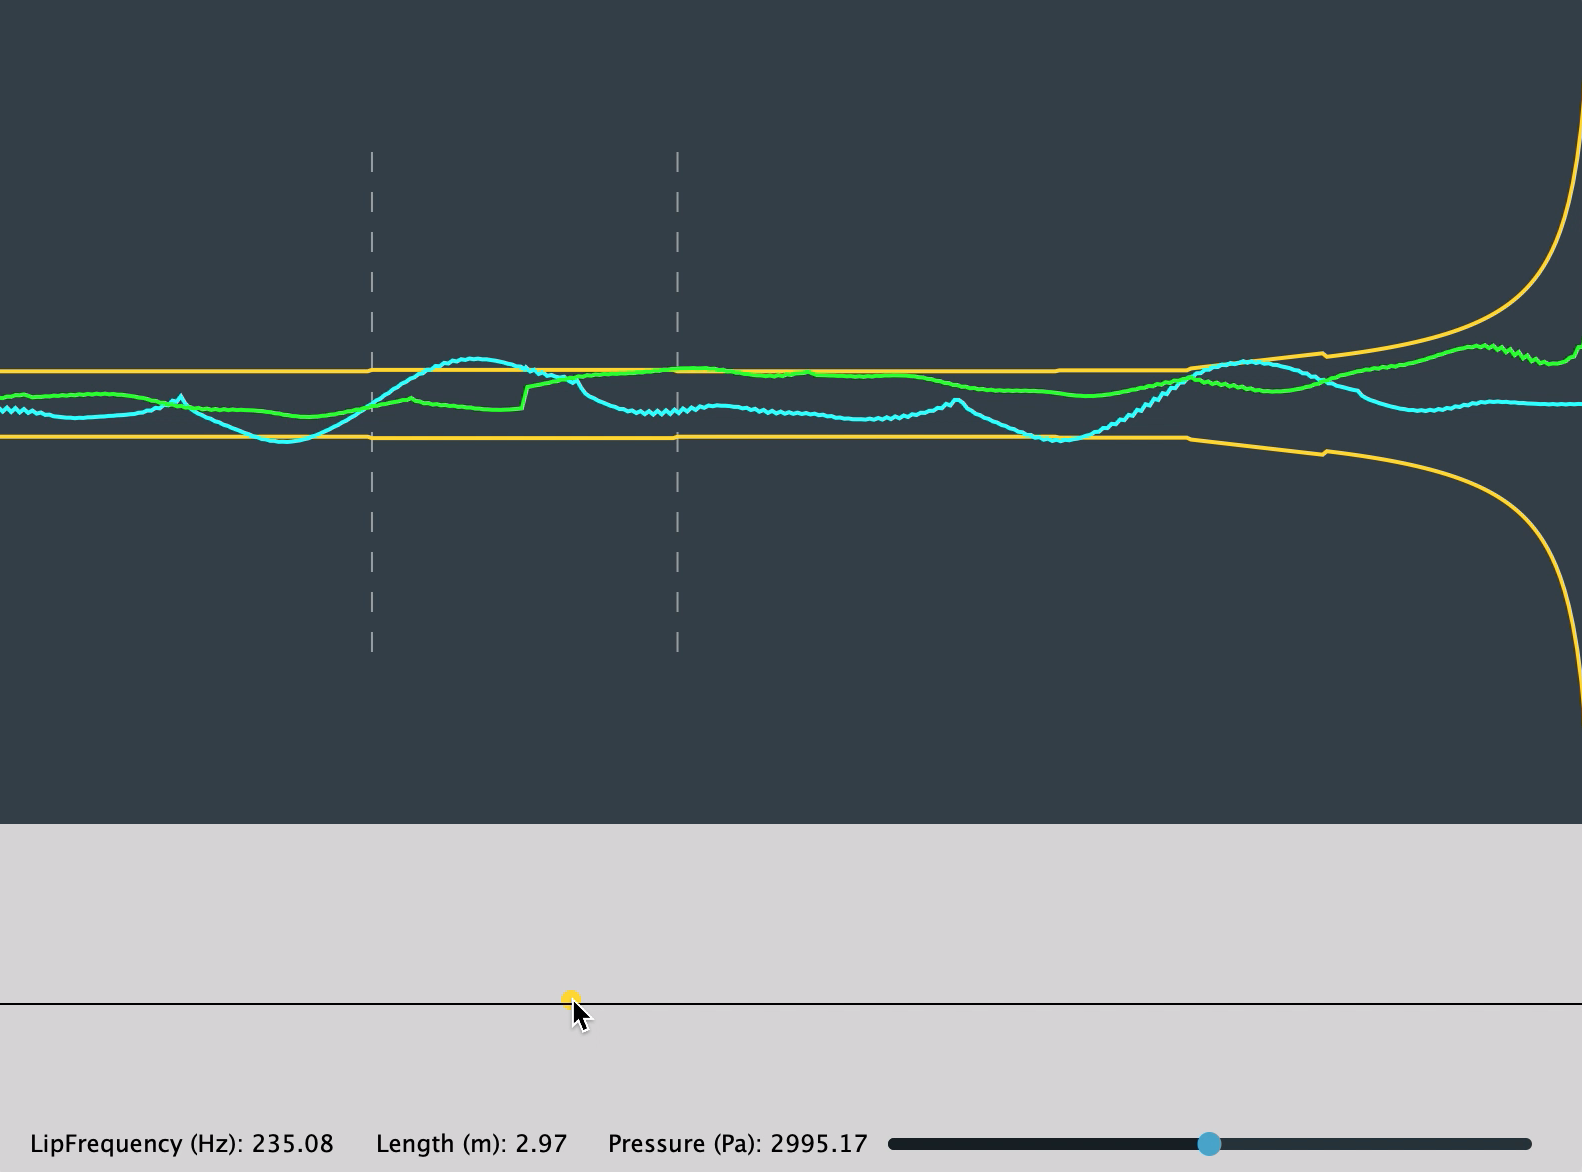
\includegraphics[width = 0.9\columnwidth]{Figures/GUI.png}}
    \caption{Screenshot of the graphical user interface. The geometry as well as the states of the pressure (in blue) and velocity scaled by $S$ (in green) are shown. For clarity, the start and end of the outer slide is denoted by dashed lines. The drift of $w$ is visible from the ``kink'' in the green line right in the middle of the outer slide.}
    \label{fig:GUI}
\end{figure}

The rest of this section provides the parameter values used in the simulation after which different aspects of the implementation that require extra attention are highlighted.

\subsection{Parameters}
For the most part, the parameters used in the simulation have been obtained from \cite{Harrison2018, Smyth2011, Benade1968}. The lengths and radii of different parts of the tube can be found in Table \ref{tab:geometry} and a diagram showing this geometry is shown in Figure \ref{fig:tromboneSchematic}.
The system is split at the end of the trombone slide such that the ranges for the lengths of the two tubes are $L_p^n \in[0.797, 1.327]$ and $L_q^n \in [1.796, 2.326]$.

Other parameters used in the simulation can be found in Table \ref{tab:parameters}. Not included here, is $\lambda$ which has been set slightly lower than the stability condition in \eqref{eq:CFL}, i.e., $\lambda = 0.999$. Although the implementation works when $\lambda = 1$, this is done to tolerate (much) higher speeds of change in $L^n$ before instability occurs (see Section \ref{sec:limit}). Not satisfying condition \eqref{eq:CFL} causes bandlimiting and dispersive effects \cite{bilbao2009}, but such a small deviation from the condition has no audible influence on the output sound and outweighs the problems caused by instability.

As the tube acts mainly as an amplifier for specific resonant frequencies it is important to match the frequency of the lip reed to a resonating mode of the tube, which depends on $L^n$ in the following way
\begin{equation}
    \omega_0^{n+1/2} = \mathcal{F}\frac{2\pi c}{\rho_0 L^{n+1/2}}
\end{equation}
where $L^{n+1/2} = L^n$ and scalar multiplier $\mathcal{F} \approx 2.4$ \SWcomment[double check this] was heuristically found to best match the 4\textsuperscript{th} resonating mode of the tube and generates a recognisable brass sound.
\begin{table}[t]
    \small
    \begin{center}
    \begin{tabular}{|l|c|c|}
        \hline
        Part of tube & Length (cm) & Radius (cm)\\\hline
        Inner slide (1) & 70.8 & 0.69\\
        Outer slide (extended) (2) & 53 & 0.72 
        \\
        Slide crook (3)& 17.7 & 0.74\\
        Outer slide (extended) (4) & 53 & 0.72 
        \\
        Inner slide (5) & 71.1 & 0.69\\
        Gooseneck (6) & 24.1 & 0.71\\
        Tuning slide (7) & 25.4 & 0.75, 1.07\\
        Bell flare (8) & 50.2& 1, 10.8\\\hline
    \end{tabular}
    \caption{Geometry of a measured trombone taken from \cite{Smyth2011}. Numbers correspond to Figure \ref{fig:tromboneSchematic}.\label{tab:geometry}}
    \end{center}
\end{table}

\begin{figure}[ht]
    \centering
    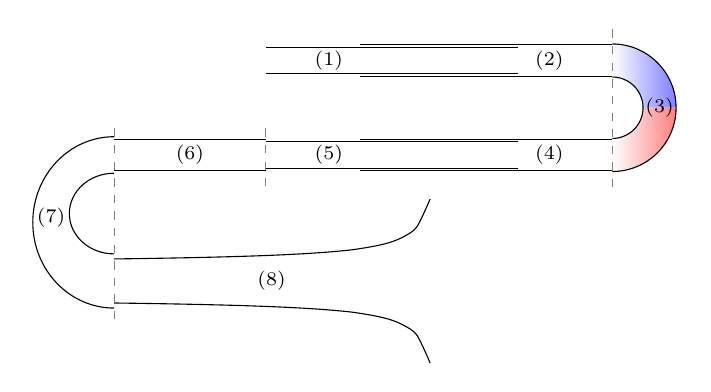
\begin{tikzpicture}[scale = 8]

    \def\labelColor{black};
    \def\labelSize{\fontsize{7pt}{7pt}\selectfont};

    \def\hornOffset{0.025};
    \def\stepSize{0.004}

    \def\dashedLineColor{gray};
    \def\dashedLineOvershoot{0.025}
    % tuning slide params
    \def\tuningSlideDim{0.1};
    \pgfmathsetmacro{\tuningSlideRad}{\stepSize + \hornOffset};
    \def\tuningSlideOffset{0.007};

    % gooseneck params
    \def\gooseNeckLength{0.241};
    \pgfmathsetmacro{\gooseNeckRad}{\tuningSlideRad - \stepSize};

    % inner slide params
    \def\innerLength{0.4};
    \pgfmathsetmacro{\innerRad}{\gooseNeckRad - \stepSize};

    % outer slide params
    \def\outerLength{\innerLength};
    \pgfmathsetmacro{\outerRad}{\gooseNeckRad};
    \pgfmathsetmacro{\extension}{0.15};

    \def\endOfSlideDim{0.075};
    \pgfmathsetmacro{\endOfSlideRad}{\outerRad * 1.05};

    %% draw horn

    \draw[domain=0:0.502, smooth, variable=\x, black] plot ({\x}, {\hornOffset + 0.0063 * ((0.502-\x) + 0.0174)^(-0.7)});
    
    \draw[domain=0:0.502, smooth, variable=\x, black] plot ({\x}, {-\hornOffset-0.0063 * ((0.502-\x) + 0.0174)^(-0.7)});
    
    \node[anchor = center, color = \labelColor](eight) at (0.25, 0) {\labelSize(8)};

    % draw tuningSlide
    \pgfmathsetmacro{\innerTuningSlideDim}{(\tuningSlideDim - \tuningSlideRad)}
    \pgfmathsetmacro{\outerTuningSlideDim}{(\tuningSlideDim + \tuningSlideRad)}

    \node[anchor = center, color = \labelColor](seven) at (-\innerTuningSlideDim-\tuningSlideRad, \innerTuningSlideDim+\tuningSlideRad) {\labelSize(7)};

    \pgfmathsetmacro{\innerTuningSlideWithOffset}{\innerTuningSlideDim - \tuningSlideOffset}

    \pgfmathsetmacro{\outerTuningSlideWithOffset}{\outerTuningSlideDim + \tuningSlideOffset}

    \draw (0, 2*\tuningSlideDim-\tuningSlideRad) arc(90:270:\innerTuningSlideDim cm and \innerTuningSlideWithOffset cm);

    \draw (0, 2*\tuningSlideDim+\tuningSlideRad) arc(90:270:\outerTuningSlideDim cm and \outerTuningSlideWithOffset cm);
    
    % dashedline
    \draw[dashed, color = \dashedLineColor] (0, -\tuningSlideRad-\tuningSlideOffset-\dashedLineOvershoot) -- (0, 2*\tuningSlideDim+\tuningSlideRad+\dashedLineOvershoot);

    % draw gooseneck
    \draw (0, 2*\tuningSlideDim + \gooseNeckRad) -- (\gooseNeckLength, 2*\tuningSlideDim + \gooseNeckRad);

    \draw (0, 2*\tuningSlideDim - \gooseNeckRad) -- (\gooseNeckLength, 2*\tuningSlideDim - \gooseNeckRad);

    \node[anchor = center, color = \labelColor](six) at (0.5 * \gooseNeckLength, 2*\tuningSlideDim) {\labelSize(6)};

    % dashedline
    \draw[dashed, color = \dashedLineColor] (\gooseNeckLength, 2*\tuningSlideDim-\gooseNeckRad-\dashedLineOvershoot) -- (\gooseNeckLength, 2*\tuningSlideDim+\gooseNeckRad+\dashedLineOvershoot);

    % draw inner slide
    \draw (\gooseNeckLength, 2*\tuningSlideDim + \innerRad) -- (\gooseNeckLength+\innerLength, 2*\tuningSlideDim + \innerRad);

    \draw (\gooseNeckLength, 2*\tuningSlideDim - \innerRad) -- (\gooseNeckLength+\innerLength, 2*\tuningSlideDim - \innerRad);

    \node[anchor = center, color = \labelColor](five) at (\gooseNeckLength + 0.25 * \innerLength, 2*\tuningSlideDim) {\labelSize(5)};

    % draw outer slide
    \pgfmathsetmacro{\outerSlideStart}{\gooseNeckLength + \extension};

    \draw (\outerSlideStart, 2*\tuningSlideDim + \outerRad) -- (\outerSlideStart+\outerLength, 2*\tuningSlideDim + \outerRad);

    \draw (\outerSlideStart, 2*\tuningSlideDim - \outerRad) -- (\outerSlideStart+\outerLength, 2*\tuningSlideDim - \outerRad);

    \node[anchor = center, color = \labelColor](four) at (\outerSlideStart + 0.75 * \outerLength, 2*\tuningSlideDim) {\labelSize(4)};


    % draw end of slide
    
    \pgfmathsetmacro{\innerEndOfSlideDim}{(\endOfSlideDim - \endOfSlideRad)};
    \pgfmathsetmacro{\outerEndOfSlideDim}{(\endOfSlideDim + \endOfSlideRad)};

    \pgfmathsetmacro{\startEndOfSlide}{\outerSlideStart + \outerLength};
    % division blue
    \fill[white, left color=white, right color=blue, fill opacity = 0.5] 
    (\startEndOfSlide+\innerEndOfSlideDim,2*\tuningSlideDim+\endOfSlideDim) 
    arc (0:90:\innerEndOfSlideDim cm and \innerEndOfSlideDim cm) 
    -- (\startEndOfSlide,2*\tuningSlideDim+\endOfSlideDim + \innerEndOfSlideDim)
    -- (\startEndOfSlide,2*\tuningSlideDim+2*\endOfSlideDim+\endOfSlideRad)
    arc (90:0:\outerEndOfSlideDim cm and \outerEndOfSlideDim cm)
    -- (\startEndOfSlide+\outerEndOfSlideDim,2*\tuningSlideDim+\endOfSlideDim)
    -- cycle;

    % division red
    \fill[white, left color=white, right color=red, fill opacity = 0.5] 
    (\startEndOfSlide+\innerEndOfSlideDim,2*\tuningSlideDim+\endOfSlideDim) 
    arc (0:-90:\innerEndOfSlideDim cm and \innerEndOfSlideDim cm) 
    -- (\startEndOfSlide,2*\tuningSlideDim+\endOfSlideDim)
    -- (\startEndOfSlide,2*\tuningSlideDim-\endOfSlideRad)
    arc (-90:0:\outerEndOfSlideDim cm and \outerEndOfSlideDim cm)
    -- (\startEndOfSlide+\outerEndOfSlideDim,2*\tuningSlideDim+\endOfSlideDim)
    -- cycle;

    \draw (\startEndOfSlide, 2*\tuningSlideDim+\endOfSlideRad) arc(-90:90:\innerEndOfSlideDim cm and \innerEndOfSlideDim cm);

    \draw (\startEndOfSlide, 2*\tuningSlideDim-\endOfSlideRad) arc(-90:90:\outerEndOfSlideDim cm and \outerEndOfSlideDim cm);

    \node[anchor = center, color = \labelColor](three) at (\startEndOfSlide + \innerEndOfSlideDim + \endOfSlideRad, 2*\tuningSlideDim+ \innerEndOfSlideDim + \endOfSlideRad) {\labelSize(3)};


    % dashedline
    \draw[dashed, color = \dashedLineColor] (\startEndOfSlide, 2*\tuningSlideDim-\endOfSlideRad-\dashedLineOvershoot) -- (\startEndOfSlide, 2*\tuningSlideDim+2*\endOfSlideDim+\endOfSlideRad+\dashedLineOvershoot);

    % draw second outer slide

    \draw (\outerSlideStart, 2*\tuningSlideDim + 2 * \endOfSlideDim + \outerRad) -- (\outerSlideStart+\outerLength, 2*\tuningSlideDim + 2 * \endOfSlideDim + \outerRad);

    \draw (\outerSlideStart, 2*\tuningSlideDim + 2 * \endOfSlideDim - \outerRad) -- (\outerSlideStart+\outerLength, 2*\tuningSlideDim + 2 * \endOfSlideDim - \outerRad);

    \node[anchor = center, color = \labelColor](two) at (\outerSlideStart + 0.75 * \outerLength, 2*\tuningSlideDim + 2 * \endOfSlideDim) {\labelSize(2)};

    % draw inner slide
    \draw (\gooseNeckLength, 2*\tuningSlideDim+ 2 * \endOfSlideDim + \innerRad) -- (\gooseNeckLength+\innerLength, 2*\tuningSlideDim+ 2 * \endOfSlideDim + \innerRad);

    \draw (\gooseNeckLength, 2*\tuningSlideDim + 2 * \endOfSlideDim - \innerRad) -- (\gooseNeckLength+\innerLength, 2*\tuningSlideDim + 2 * \endOfSlideDim - \innerRad);

    \node[anchor = center, color = \labelColor](one) at (\gooseNeckLength + 0.25 * \innerLength, 2*\tuningSlideDim + 2 * \endOfSlideDim) {\labelSize(1)};

% \begin{scope}[very thick,decoration={
%     markings,
%     mark=at position 0.5 with {\arrow{>}}}
%     ] 
%     \draw[postaction={decorate}] (-4,0)--(4,0);
% \end{scope}
    
    \end{tikzpicture}
    \caption{Schematic of the trombone. Numbers correspond to the parts of the tube found in Table \ref{tab:geometry} and dashed lines highlight where parts are separated. The scheme is split in the middle of the slide crook with the colours corresponding to those in \ref{fig:dynamicGridSchematic}.}
    \label{fig:tromboneSchematic}
\end{figure}

\begin{table}[t]
    \small
    \begin{center}
    \begin{tabular}{|l|c|c|}
        \hline
        Name & Symbol (unit) & Value\\ \hline
        \multicolumn{3}{|l|}{\bf Tube}\\ \hline
        Length & $L$ (m) & $2.593\leq L \leq 3.653$$^\star$\\
        Air density &$\rho_0$ (kg/m$^3$) & 1.1769** 
        \\
        Wave speed & $c$ (m/s) & 347.23**\\
        Geometry & $S$ (m$^2$) & See Table \ref{tab:geometry}. \\\hline
        \multicolumn{3}{|l|}{\bf Lip reed}\\ \hline
        Mass & $M_\text{r}$ (kg) & $5.37\cdot10^{-5}$*\\
        Frequency & $\omega_0$ (rad/s) & $ 50\leq \omega_0/2\pi \leq 1000$\\
        Mouth pressure & $P_\text{m}$ (Pa) & $0 \leq P_\text{m} \leq 6000$\\
        Damping & $\sigma_\text{r}$ (s$^{-1}$) & $5$*\\
        Eff. surface area & $S_\text{r}$ (m$^{2}$) & $1.46\cdot 10^{-5}$*\\
        Width & $w_\text{r}$ (m) & $0.01$* \\
        Equilibrium sep. & $H_0$ (m) &  $2.9 \cdot 10^{-4}$* \\
        Coll. stiffness& $K_\text{c}$ (N/m) & $10^4$\\
        Nonlin. coll. coeff.& $\alpha_\text{c}$ (-)  &3\\\hline
        \multicolumn{3}{|l|}{\bf Other}\\ \hline
        State corr. stiffness & $\omega_\text{sc}$ & $1$\\ 
        State corr. damping & $\sigma_\text{sc}$ & $1$\\ 
        Sample rate & $f_\text{s}$ (Hz) & 44100\\
        \hline
    \end{tabular}
    \caption{List of parameter values used for the simulation. 
    Taken from $^\star$\cite{Smyth2011}, *\cite{Harrison2018} or **\cite{Benade1968} with temperature $T=26.85^\circ C$. \label{tab:parameters}}
    \end{center}
\end{table}

The output of the system can be retrieved by selecting a grid point on the pressure grid and listening to this at the given sample rate $f_\text{s}$. The most logical would be to listen to the rightmost grid point, i.e., the radiating boundary $q_{M_q}^n$ as this is also where the sound enters the listening space in the real world. 

\subsection{Limit on speed of change}\label{sec:limit}
To reduce audible artefacts and instability issues from adding and removing points \SWcomment[and to also stay in the sub-audio rate regime], a limit can be placed on \eqref{eq:lDiff} as
\begin{equation}\label{eq:Nmaxdiff} 
    L_\text{diff}^n \leq \Nfrac_\text{maxdiff} h
\end{equation}
where $\Nfrac_\text{maxdiff}$ is the maximum change in $\Nfrac$ per sample and has been set to $\Nfrac_\text{maxdiff} = 1/20$. This means that a grid point can be added or removed every 20 samples and allows the entire range of $L$ to be traversed in ca. 0.06 s at a sample rate of $f_\text{s} = 44100$ Hz. \SWcomment[still sub-audio rate though?]

\subsection{State correction}\label{sec:impStateCorr}
The centred operators in Eq. \eqref{eq:scForce} and with that the introduction of states at $n+1$ seem to make the scheme implicit. It is, however, possible to calculate $F_\text{sc}$ explicitly \cite{bilbao2009, bilbao2009dafx}. The same also introduce the need for values at $n-1$, i.e., $p_{M}^{n-1}$ and $q_{0}^{n-1}$. Therefore, the vectors $\mathbf{p}^{n-1}$ and $\mathbf{q}^{n-1}$ will need to be stored, and the operations to add and remove grid points as described in \ref{sec:addRemove} need to be applied to these as well. One could argue that only two points at the inner boundaries are needed to create $\mathbf{r}^{n-1}$, but for generality, we continue with the entire vectors defined over the same domains as $\mathbf{p}^n$ and $\mathbf{q}^{n}$ respectively. 

\subsection{Order of Calculation}

Algorithm \ref{alg:calcOrder} shows pseudocode showing the order in which the different parts of the system presented in this paper are calculated.
\begin{algorithm}[ht]
    \setstretch{1.1}
    \fbox{\parbox{0.88\linewidth}
    {
        \While{application is running}
        {
            \begin{minipage}[c]{0.48\linewidth}
                Retrieve new parameters\\
                Update $L_p^n$ and $L_q^n$\\
                Calc. $\Nfrac^n$ and $N^n$\\
                Calc. $\alpha$ \\
                \If{$ N^n \neq N^{n-1} $}
                {
                    Add or remove point\\
                    Update $M$ and $M_q$ 
                }
                Calc. $p_{M+1}^n$ and $q_{-1}^n$ \\
                Calc. $\mathbf{v}^{n+1/2}$ and  $\mathbf{w}^{n+1/2}$ \\
                Calc. $y^{n+3/2}$ w/o collision \\
                Calc $g^{n+1/2}$ \\
                Calc. $y^{n+3/2}$ with collision \\
                Calc. $U_\text{B}^{n+1/2}$ and $U_\text{r}^{n+1/2}$ \\
                Calc. $\mathbf{p}^{n+1}$ and $\mathbf{q}^{n+1}$ \\
                Retrieve output
            \end{minipage}
            \begin{minipage}[c]{0.43\linewidth}
                ($L^n$, $\omega_0^n$ and $P_\text{m}^n$) \\
                (Eqs. \eqref{eq:lDiff}, \eqref{eq:Nmaxdiff} \& \eqref{eq:updateLs})\\
                (Eqs. \eqref{eq:nfrac} and \eqref{eq:numberOfIntervals})\\
                (Eq. \eqref{eq:alphaDef})\\
                \vspace{-0.2em}\\
                (Eq. \eqref{eq:addingPoint} or \eqref{eq:removingPoint})\\
                (Eq. \eqref{eq:MMq})\\
                \vspace{-0.15em}\\
                (Eqs. \eqref{eq:connectionInterpol})\vspace{0.05em}\\
                (Eqs. \eqref{eq:discVelocityV} and \eqref{eq:discVelocityW})\\
                (Eqs. \eqref{eq:discreteLipSystem})\\
                (Eq. \eqref{eq:gDef})\\
                (Eqs. \eqref{eq:discreteLipSystem})\\
                (Eqs. \eqref{eq:bernoulli} and \eqref{eq:Ur})\\
                (Eqs. \eqref{eq:pressuresWithSC})
                \vspace{0.25em}\\
           \end{minipage}
           \\
           \begin{minipage}[c]{0.4\linewidth}
                Update system states\\
                \\
                \\
                Update $N$ \\
                Increment $n$      
            \end{minipage}
            \begin{minipage}[c]{0.5\linewidth}
                ($\mathbf{p}^{n-1} = \mathbf{p}^{n}$, $\mathbf{p}^n=\mathbf{p}^{n+1}$)
                (same for $\mathbf{v}^{n-1/2} = \hdots$,\\
                $y^{n-1/2}$, $y^{n+1/2}$, and $\psi^n$)\\
                ($N^{n-1} = N^n$)\\
            \end{minipage}
            }
        }
    }
    \vspace{0.12cm}
    \caption{Pseudocode showing the order of calculations of the algorithm implementing the trombone .\label{alg:calcOrder}}
\end{algorithm}

% \begin{algorithm}[ht]
%     \setstretch{1.1}
%     \fbox{\parbox{0.88\linewidth}
%     {
%         \While{application is running}
%         {
%             Retrieve new parameters ($L^n$, $\omega_0^n$ and $P_\text{m}^n$) \\
%             Update $L_p^n$ and $L_q^n$ (Eqs. \eqref{eq:lDiff}, \eqref{eq:Nmaxdiff} and \eqref{eq:updateLs})\\
%             Calc. $\Nfrac^n$ and $N^n$ (Eqs. \eqref{eq:nfrac} and \eqref{eq:numberOfIntervals}) \\
%             Calc. $\alpha$ (Eq. \eqref{eq:alphaDef})\\
%             \If{$ N^n \neq N^{n-1} $}
%             {
%                 Add or remove point (Eq. \eqref{eq:addingPoint} or \eqref{eq:removingPoint})\\
%                 Update $M$ and $M_q$ (Eq. \eqref{eq:MMq})
%             }
%             Calc. $p_{M+1}^n$ and $q_{-1}^n$ (Eqs. \eqref{eq:connectionInterpol})\\
%             Calc. $\mathbf{v}^{n+1/2}$ and  $\mathbf{w}^{n+1/2}$ (Eqs. \eqref{eq:discVelocityV} and \eqref{eq:discVelocityW})\\
%             Calc. $y^{n+3/2}$ w/o collision (Eqs. \eqref{eq:discreteLipSystem})\\
%             Calc $g^{n+1/2}$ (Eq. \eqref{eq:gDef})\\
%             Calc. $y^{n+3/2}$ with collision (Eqs. \eqref{eq:discreteLipSystem})\\
%             Calc. $U_\text{B}^{n+1/2}$ and $U_\text{r}^{n+1/2}$ (Eqs. \eqref{eq:bernoulli} and \eqref{eq:Ur})\\
%             Calc. $\mathbf{p}^{n+1}$ and $\mathbf{q}^{n+1}$ (Eqs. \eqref{eq:pressuresWithSC})\\ 
%             Retrieve output\\
%             Update system states ($\mathbf{p}^{n-1} = \mathbf{p}^{n}$, $\mathbf{p}^n=\mathbf{p}^{n+1}$)\\
%             (same for $\mathbf{v}^{n-1/2} = \hdots$, $y^{n-1/2}$, $y^{n+1/2}$, and $\psi^n$),\\
%             % \begin{minipage}[c]{0.4\linewidth} 
%             % Update system states\\
%             % \\
%             % \\
%             % \\
%             % \end{minipage} \begin{minipage}[c]{0.5\linewidth} 
%             % $\mathbf{p}^{n-1} = \mathbf{p}^n$, $\mathbf{p}^n = \mathbf{p}^{n+1}$,\\
%             % $\mathbf{v}^{n-1/2} = \mathbf{v}^{n+1/2}$,\\
%             % $y^{n-1/2} = y^{n+1/2}$,\\
%             % $y^{n+1/2} = y^{n+3/2}$, \\
%             % $\psi^{n} = 
%             % \psi^{n+1}$, 
%             % \end{minipage}\\
%             Update $N$ ($N^{n-1} = N^n$)\\
%             Increment $n$            % \begin{minipage}[c]{0.4\linewidth}
%             % -\\
%             % \vspace{2em}(Eq. \eqref{eq:addingPoint})\\
            
%             % (Eq. \eqref{eq:removingPoint})\\

%             % \end{minipage}
%             }
%         }
%     }
%     \vspace{0.12cm}
%     \caption{Pseudocode showing the order of calculations of the algorithm implementing the trombone .\label{alg:calcOrder}}
% \end{algorithm}

